\documentclass[12pt, onesided]{article}
\usepackage[latin1]{inputenc}
\usepackage[margin=0.5in]{geometry}
%\usepackage[dvips]{graphics, color}
%\usepackage{tikz}
%\usepackage{tkz-berge}
\usepackage[pdftex]{graphicx, color}
\usepackage{pictex}
\usepackage{amsmath}
\usepackage{amsthm}
\usepackage{amsfonts}
\usepackage{amssymb}
\usepackage{bm}
\usepackage{mathrsfs}
\usepackage{verbatim}
\usepackage{hyperref}
\usepackage{enumerate}
\usepackage{listings}
\setcounter{MaxMatrixCols}{15}


\providecommand{\SetFigFont}[6]{$\scriptstyle{#6}$}



%%%%%%%%%%%%%%%%%%%%%%%%%%%%%%%%%%%%%%%%%%%%%%%%%%%%%%%%%%%
%    Macros


%Greek letters
\providecommand{\D}{\Delta}
\renewcommand{\S}{\Sigma}
\providecommand{\G}{\Gamma}
\renewcommand{\a}{\alpha}
\renewcommand{\b}{\beta}
\renewcommand{\t}{\theta}
\providecommand{\g}{\gamma}
\renewcommand{\d}{\delta}
%\providecommand{\e}{\varepsilon}
\renewcommand{\th}{\theta}
\renewcommand{\l}{\lambda}
\renewcommand{\L}{\Lambda}
\renewcommand{\O}{\Omega}
\providecommand{\s}{\sigma}
\providecommand{\g}{\gamma}
\providecommand{\vp}{\varphi}
\renewcommand{\o}{\omega}
\renewcommand{\t}{\tau}
\newcommand{\var}{\text{var}}



%Blackboard symbols:
\newcommand{\R}{\mathbb R}
\renewcommand{\P}{\mathbb P}
\newcommand{\T}{\mathscr T}
\newcommand{\N}{\mathbb N}
\newcommand{\Z}{\mathbb Z}
\newcommand{\BO}{\mathcal{O}}
\newcommand{\CD}{\mathscr{D}}
\newcommand{\sN}{\mathscr{N}}
\newcommand{\sn}[1]{\mathscr{N}_{#1}}
\newcommand{\sM}{\mathscr{M}}
\newcommand{\sG}{\mathscr{G}}
\newcommand{\F}{\mathscr{F}}
\newcommand{\sL}{\mathscr{L}}
\newcommand{\p}{\rho}
\newcommand{\Y}{\textbf{Y}}
\newcommand{\X}{\textbf{X}}
\newcommand{\w}{\textbf{w}}
\newcommand{\tw}{ \boldsymbol{ \tilde w}}
\renewcommand{\th}{\theta}
\renewcommand{\r}{\textbf{r}}
\newcommand{\E}{\boldsymbol{\epsilon}}
\newcommand{\B}{\boldsymbol{\beta}}
\renewcommand{\b}{\boldsymbol{\beta}}
\providecommand{\e}[1]{\ensuremath{\times 10^{#1}}}

%New symbols
\DeclareMathOperator{\dep}{dep}




%%%%%%%%%%%%%%%%%%%%%%%%%%%%%%%%%%%%%%%%%%%%%%%%%%%%%%%%%%%
%	Theorem-like environments

	%\newtheorem{theorem}{Theorem}
	%\newtheorem{lemma}{Lemma}
	%\newtheorem{definition}{Definition}
	%\newtheorem{corollary}{Corollary}
	%\newtheorem{example}{Example}
	%\newtheorem{notation}{Notation}

%This numbers the theorems, lemmas and corollaries
%according to the same scheme.

\newtheorem{theorem}{Theorem}[section]
\newtheorem{lemma}[theorem]{Lemma}
\newtheorem{corollary}[theorem]{Corollary}

\newtheorem{example}{Example}
\newtheorem{notation}{Notation}
\newtheorem{definition}{Definition}

%This will print the equation numbers according
%to sections.

\renewcommand{\theequation}
	{\arabic{section}.\arabic{equation}}


%%%%%%%%%%%%%%%%%%%%%%%%%%%%%%%%%%%%%%%%%%%%%%%%%%%%%%%%%%%
%    The body of the paper


\title{Forecasting the 2019 Flu Season Using Bayesian Spatial Modeling }
\author{Aaron Moose, Katie Jurewicz, and Maddy St. Ville}
\date{\today}
%\keywords{here they are}

\begin{document}

 \maketitle
% \newpage
\begin{abstract}
This paper forecasts the 2019 monthly flu season for each state in the United States, with the exception of Alaska, Florida, and Hawaii. The monthly proportion of patients diagnosed with "influenza-like-illnesses" for each state was treated as the response and was modeled using a Bayesian spatial Conditional Autoregressive (CAR) model. Markov Chain Monte Carlo sampling techniques were utilized to generate a sample used to predict the monthly number of flu cases, and modeling techniques were verified by performing several model diagnostics procedures. 
\end{abstract}
\newpage
%$\newline$
\begin{flushleft}
\section{Introduction}
Influenza - the flu - is a contagious respiratory disease that comes as a result of influenza viruses. The two common types of influenza viruses, Types A and B, are the main virus strains that cause yearly seasonal flu epidemics  \cite{CDC}. These flu epidemics result in up to 5 million severe cases and up to 500,000 deaths globally each year \cite{WHO}. Although there are cases of the flu year round in the United States, pandemics are most common during the fall and winter. The number of cases tends to increase in October, with peaks in the winter months \cite{CDC}. 
$\newline$
\\
The ultimate goal of this paper is to forecast the monthly proportion of flu cases for each state in order to predict peak flu activity. As flu epidemics typically see a fall/winter seasonality in the United States, studies have shown that the transmission of influenza viruses is dependent on the climate \cite{Lowen}. Hence, it is expected that neighboring states, with similar monthly climate conditions, will have similar peak flu months; i.e., there is most likely a spatial correlation in the monthly results. Therefore, a Conditional Autoregressive (CAR) model was fit to model the spatial effects. For covariate/predictor information, the model includes monthly climate information, demographic information, and flu history for each state. All covariate information has monthly observations from 2010-2018. The model was fit using MCMC methods. 
$\newline$
$\newline$
\section{Methodology}
\subsection{The Model}
After removing data for Alaska, Florida, and Hawaii, we are taking observations on 47 spatial units. To capture the relationship between the observations and areal units, we fit a CAR model given by
$$\boldsymbol{y}=\boldsymbol{X}\boldsymbol{\beta}+\boldsymbol{G}\boldsymbol{b}+\boldsymbol{\epsilon}.$$
Define $\boldsymbol{y}=(\boldsymbol{y}_{1},\dots ,\boldsymbol{y}_{m})$ such that $\boldsymbol{y}_{j}$ is a vector representing flu cases for the $j^{\text{th}}$ state from October 2010 to September 2018, where $y_{ijk}$ denotes the proportion of flu cases in the $i^{\text{th}}$ state during the $j^{\text{th}}$ month and $k^{\text{th}}$ year. \\

Let $\boldsymbol{X}$ and $\boldsymbol{\beta}$ denote the design matrix and regression coefficients, respectively, associated with the fixed effects. Further, $\boldsymbol{G}$ denotes the design matrix associated with spatial random effects, and $\boldsymbol{b}$ is the corresponding spatial random effects vector with $b_i$ representing the spatial random effect for the $i^{\text{th}}$ state. Finally, we assume that $\boldsymbol{y}$ follows a normal distribution; i.e.,
$$\boldsymbol{y}\sim N(\boldsymbol{X}\boldsymbol{\beta}+\boldsymbol{G}\boldsymbol{b}, \sigma^2 \boldsymbol{I}).$$
$\newline$
The following prior distributions were assigned:
\begin{equation*}
\begin{split}
\boldsymbol{\beta}&\sim N(0,R)\\
\boldsymbol{b}&\sim \text{CAR}(\tau^2,\rho) \implies \boldsymbol{b}\sim N(0, \tau^2(D-\rho W)^{-1})\\
\sigma^{-2}&\sim \text{Gamma}(a_\sigma ,b_\sigma)\\
\tau^{-2}&\sim \text{Gamma}(a_\tau ,b_\tau)\\
\end{split}
\end{equation*}
Here, $W$ represents the $47\times 47$ adjacency matrix, and $D$ is a $47\times 47$ diagonal matrix whose $i^{\text{th}}$ diagonal entry is the number of neighboring states the $i^{\text{th}}$ state has. We assume the correlation parameter, $\rho$, to be fixed. 
$\newline$
\\
The full conditional distributions were derived and are provided below where $n$ is the length of the vector $\mathbf{y}$ and $m$ is then number of states, 47.
$\newline$
$\newline$
\begin{equation*}
\begin{split}
p(\boldsymbol{\beta}|\sigma^2 , \boldsymbol{y}, \boldsymbol{b})&\sim N\left((\boldsymbol{X}^T\boldsymbol{X}+\sigma^2 R^{-1})^{-1}\boldsymbol{X}^T(\boldsymbol{y}-\boldsymbol{Gb}),\sigma^2(\boldsymbol{X}^T\boldsymbol{X}+\sigma^2 R^{-1})^{-1}\right)\\
p(\boldsymbol{b}|\sigma^2, \tau^2, \boldsymbol{y},\boldsymbol{\beta}) &\sim N\left(\left(\boldsymbol{G}^T\boldsymbol{G}+\sigma^2\frac{(D-\rho W)}{\tau^2}\right)^{-1}\boldsymbol{G}^T(\boldsymbol{y}-\boldsymbol{X\beta}), \sigma^2 \left(\boldsymbol{G}^T\boldsymbol{G}+\sigma^2\frac{(D-\rho W)}{\tau^2}\right)^{-1}\right)\\
p(\sigma^{-2}|\boldsymbol{y},\boldsymbol{\beta},\boldsymbol{b})&\sim \text{Gamma}\left(a_\sigma +\frac{n}{2}, b_\sigma +\frac{1}{2}(\boldsymbol{y}-\boldsymbol{X\beta}-\boldsymbol{Gb})^T(\boldsymbol{y}-\boldsymbol{X\beta}-\boldsymbol{Gb})\right)\\
p(\tau^{-2}|\boldsymbol{b})&\sim \text{Gamma}\left(a_\tau +\frac{m}{2}, b_\tau +\frac{1}{2}\boldsymbol{b}^T(D-\rho W)\boldsymbol{b}\right)\\
\end{split}
\end{equation*}
$\newline$
$\newline$
\subsection{Fitting the Model}
The above model was fit via a full block Gibbs Sampling Algorithm. The algorithm ran for 50,000 iterations under the following procedure. 
\begin{enumerate}
\item Provide initial values for the parameters, $(\beta^{(0)}, b^{(0)}, (\sigma^{-2})^{(0)}, (\tau^{-2})^{(0)})$.
\item For $g=1,\dots ,10000$, generate from the following sequence of full conditional distributions:
\begin{enumerate}
\item Sample $\beta^{(g)}\sim p\left(\boldsymbol{\beta}|(\sigma^{-2})^{(g-1)}, b^{(g-1)}, y\right)$
\item Sample $b^{(g)}\sim p\left(\boldsymbol{b}|\beta^{(g)}, (\sigma^{-2})^{(g-1)}, (\tau^{-2})^{(g-1)}, y\right)$
\item Sample $(\sigma^{-2})^{(g)}\sim p\left(\sigma^{-2}|\beta^{(g)}, b^{(g)}, y\right)$
\item Sample $(\tau^{-2})^{(g)}\sim p\left(\tau^{-2}|b^{(g)}\right)$
\end{enumerate}
\item Reinitialize parameter values to $(\beta^{(g)}, b^{(g)}, (\sigma^{-2})^{(g)}, (\tau^{-2})^{(g)})$.
\end{enumerate}

The following hyperparameters and initial values were assigned:
\begin{equation*}
\begin{split}
 R&=100\boldsymbol{I} \\
  \boldsymbol{b}&=0\\
  \rho&= 0.9\\
  \sigma^2 &=2\\
  a_\sigma ,b_\sigma&=0\\
  \tau^2 &=2\\
  a_\tau ,b_\tau &=0.\\
\end{split}
\end{equation*}
\subsection{The Data}
We utilized previous flu history from 2010-2018 to fit the model. There are more than 2900 healthcare providers nationally that provide data to the Centers for Disease Control and Prevention (CDC) of the total number of patients seen as well as the total number of patients diagnosed with an ILI each week. With this, the CDC organizes and releases ILINet surveillance data to the public each week \cite{Osthus}. ILI refers to influenza-like illness and is defined to be a temperature of 100 degrees Fahrenheit or greater as well as a cough or sore throat with no other known cause except for influenza \cite{Osthus}. The total number of ILI patients divided by the total number of patients provides an estimate of the total population that experience an ILI. This value is not adjusted to the population of the state and is therefore an unweighted ILI estimate \cite{Overview}. The ILINet also provides a weighted ILI percentage which is weighted on the basis of state population \cite{Overview}. The weeks stated in the ILINet dataset are based on the surveillance weeks as defined by the morbidity and mortality weekly reports \cite{Biggerstaff}. 
$\newline$
\\
The unweighted ILI data was used as the response variable for the current analysis. The weighted ILI were unavailable, thus unweighted were used. The ILI data was originally in a weekly format; thus, we transformed the data based on the morbidity and mortality weekly reports calendar. Depending on if January $1^{\text{st}}$ falls in the beginning or end of the week, "week 1" data could fall into either January or December, allowing for there to be a maximum of 53 weeks in a year \cite{MMWR}.
$\newline$
\\
The full model included the following predictor variables: temperature, precipitation, population density, and unemployment as well as an intercept and indicator variables for each month, with October as the baseline. Temperature and precipitation data points refer to the averages for each month for every state \cite{Climate}. Temperature was measured in degrees Fahrenheit and precipitation was measured in inches. Population density was calculated based off of population and land area metrics for each state \cite{USCensus}. The United States Census Bureau \cite{USCensus} provided population estimates by year and land area in square miles for each state; thus, population density was calculated as the number of people in the state per square mile. Lastly, unemployment data refers to the unemployment rate for each month in every state \cite{LaborStat}. Data from years 2010-2018 framed the current analysis. All data were on the state and monthly levels. Florida, DC, Alaska, and Hawaii were removed from all data sets and, when applicable, New York City data was combined with New York State data.
$\newline$
$\newline$
\subsection{Model Diagnostics}
Trace plots and effective sample size were utilized in performing model diagnostics. The effective sample size ranged from 139 to 46,842. Further, the following figure provides the trace plots for the components of $\boldsymbol{\beta}$, of which we can see that each component converged. 
\newpage
\begin{figure}[h!]
\centering
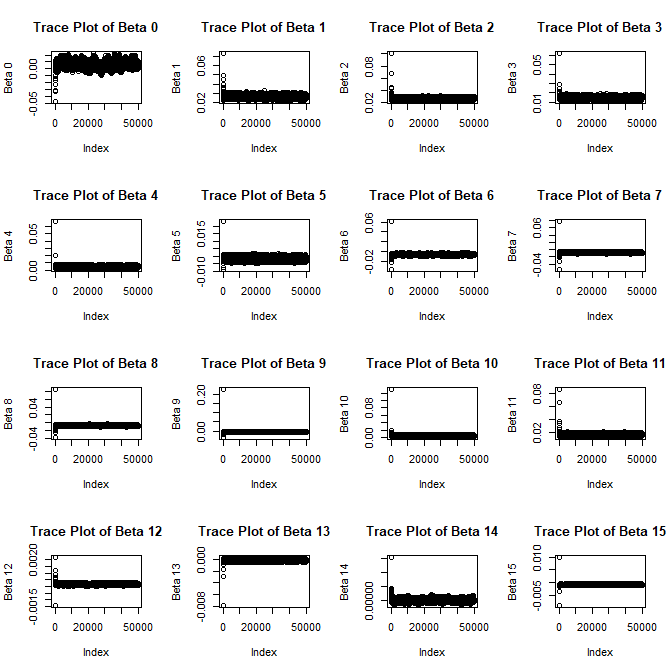
\includegraphics[scale=0.5]{Project1_traceplots}
\end{figure}
The expected mean of all the $\mathbf{\beta}$'s are
\begin{center}
\begin{tabular}{cc|cc}
$\beta_0$ & $2.821 \e{-3}$ & $\beta_1$ & $2.617 \e{-2}$ \\
$\beta_2$ & $2.637 \e{-2}$ & $\beta_3$ & $1.467\e{-2}$ \\
$\beta_4$ & $4.373 \e{-3}$ & $\beta_5$ & $-1.545\e{-2}$ \\
$\beta_6$ & $-5.548 \e{-3}$ & $\beta_7$ & $-7.784\e{-3}$ \\
$\beta_8$ & $-7.299 \e{-3}$ & $\beta_9$ & $-3.981\e{-1}$ \\
$\beta_{10}$ & $5.055 \e{-3}$ & $\beta_{11}$ & $1.617\e{-2}$ \\
$\beta_{12}$ & $1.5333 \e{-4}$ & $\beta_{13}$ & $-1.324\e{-4}$ \\
$\beta_{14}$ & $6.996 \e{-10}$ & $\beta_{15}$ & $-7.493\e{-4}$ \\
\end{tabular}
\end{center}
where $\beta_0$ to $\beta_{11}$ are the coefficients for the months. \\
In addition to this, a 95\% HPD interval was created to determine whether each $\beta_i$ was significant.
\begin{center}
\begin{tabular}{cc|cc}
$\beta_0$ & $(-0.024,0.014)$ & $\beta_1$ & $(0.024,0.029)$ \\
$\beta_2$ & $(0.024, 0.0285)$ & $\beta_3$ & $(0.013,0.016)$ \\
$\beta_4$ & $(0.003,0.006)$ & $\beta_5$ & $(-0.003,-0.00009)$ \\
$\beta_6$ & $(-0.007,-0.004)$ & $\beta_7$ & $(-0.01,-0.006)$ \\
$\beta_8$ & $(-0.009,-0.005)$ & $\beta_9$ & $(-0.006,-0.002)$ \\
$\beta_{10}$ & $(0.003,0.007)$ & $\beta_{11}$ & $(0.001,0.002)$ \\
$\beta_{12}$ & $(0.00007,0.0002)$ & $\beta_{13}$ & $(-0.0003,0.00005)$ \\
$\beta_{14}$ & $-0.00001,0.00001)$ & $\beta_{15}$ & $-0.0009,-0.0006)$ \\
\end{tabular}
\end{center}
Based off of the HPD intervals, predictors 1,14, and 15 weren't significant corresponding to the baseline $\beta_0$, the precipitation, and population density of each state. Population density is understandable, but the insignificance of the precipitation is surprising.\\

The forecast is created using the sampled values of the parameters $\boldsymbol{\beta}$ and $\boldsymbol{b}$. Choosing six particular states from different regions of the United States (South Carolina, Pennsylvania, Texas, South Dakota, Utah, and Idaho), the true values (the line) were plotted along with the predicted values (the points).
\begin{figure}[h!]
\centering
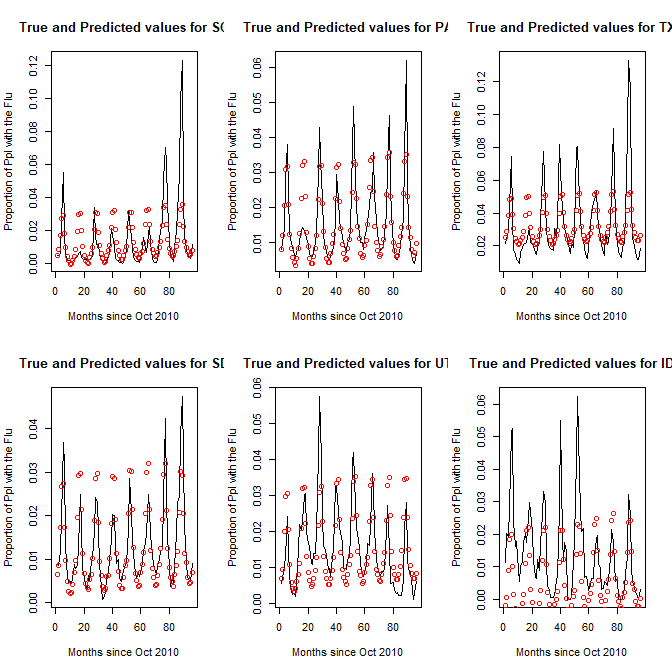
\includegraphics[width=5in, height=6in]{Project1_predict_vs_true}
\end{figure}

\section{Model Prediction}
How well does this model do in predicting the flu outbreaks in the upcoming flu season? To test this, we split our data and responses into a training and testing set where our test set is the latest flu season, October 2017 to September 2018. We then built out model on the training set and tried to predict the proportion of flu cases in the test set. Looking at the same six states as before, the predicted and true proportion of flu cases are,
\newpage
\begin{figure}[h!]
\centering
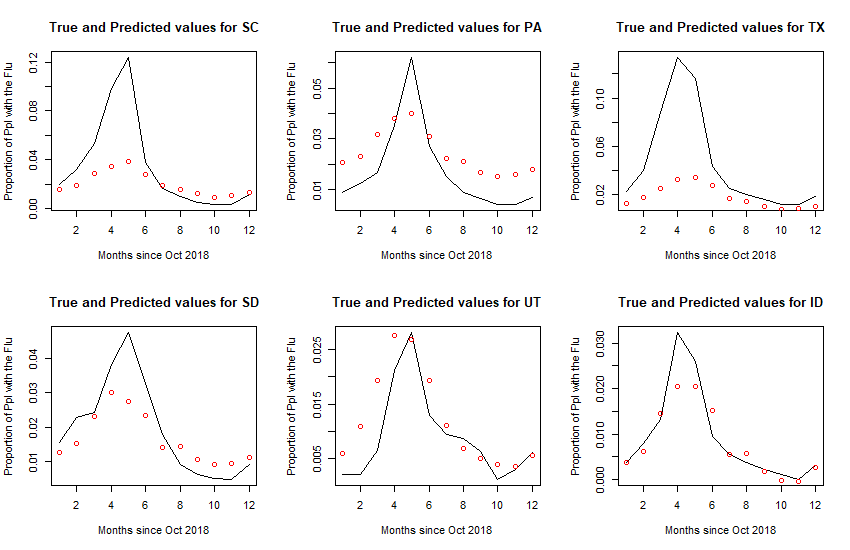
\includegraphics[scale=0.75]{TestProportionPlot}
\end{figure}

\section{Conclusion}
The model did an relatively good job at predicting the proportion of people with the flu. It was roughly split between over and under estimating the proportion of cases. To determine exactly how well they model did at predicting the proportion of flu cases, we'd need to do a goodness of fit test on all 47 states. Rather than determining how many individual cases might occur within a state, we decided to use the proportion since other models that the CDC uses have the weighted proportions as the response variables. The model did not quite predict the peaks well, but this could be because we are working with small values.\\
\indent Overall, our model did fine with only four variables, and the HPD interval removes two of those. The CDC had data on the number of people in different (and also overlapping) age groups, but the headers of each column was abbreviated and had no intuitive explanation. Since young children and the elderly are more likely to get sick, if we had at least added the number of people in those categories into the model, we would expect the model to do better. \\
\indent Another slight improvement we could do is add a Metropolis step to sample $\rho$ rather than having it fixed. The reason we did not was because every time we needed to do an inversion of a matrix, it would take too long, and with 10000 iterations, it would take up too much time to run. But, since $\rho \in [-1,1]$, we could have the proposal distribution as a reflected random walk if we wanted to do the Metropolis step.

\newpage
\lstinputlisting[language=R, breaklines=true]{Flu.R}

\end{flushleft}
\newpage
\begin{thebibliography}{9}

\bibitem{CDC}
  Centers for Disease Control and Prevention.
  \emph{Seasonal Influenza (Flu)}.
  \url{https://www.cdc.gov/flu/about/index.html}.
  Updated 2018 Oct 26.

\bibitem{WHO}
  World Health Organization.
  \emph{Influenza (Seasonal)}.
  2018.
  
\bibitem{Lowen}
Lowen A, Steel J.
\emph{Roles of Humidity and Temperature in Shaping Influenza Seasonality}.
\url{https://jvi.asm.org/content/jvi/88/14/7692.full.pdf}.
	2014 July.
	
\bibitem{Osthus}
Osthus D, Gattiker J, Priedhorsky R, Del Valle, S.
\emph{Dynamic Bayesian Influenza Forecasting in the United States with Hierarchical Discrepancy}. 
\url{https://projecteuclid.org/download/pdfview_1/euclid.ba/1533866670}.
2018.

\bibitem{Overview}
Centers for Disease Control and Prevention.
\emph{Overview of Influenza Surveillance in the United States}.
\url{https://www.cdc.gov/flu/weekly/overview.htm}.
Updated 2018 Oct 19.

\bibitem{Biggerstaff}
Biggerstaff M, Alper D, Dredze M, Fox S, Fung I, Hickmann K,....
\emph{Results from the centers for disease control and prevention's predict the 2013-2014 Influenza Season Challenge}.
\url{https://doi.org/10.1186/s12879-016-1669-x}.

\bibitem{MMWR}
Centers for Disease Control and Prevention.
\emph{MMWR Weeks}.
\url{https://wwwn.cdc.gov/nndss/document/MMWR_Week_overview.pdf}.

\bibitem{Climate}
Southern Regional Climate Center.
\emph{Monthly Summaries}.
2018.

\bibitem{USCensus}
United States Census Bureau.
\emph{State Population Totals and Components of Change: 2010-2017}.
\url{https://www.census.gov/data/tables/2017/demo/popest/state-total.html}.

\bibitem{LaborStat}
Bureau of Labor Statistics.
\emph{Local Area Unemployment Statistics}.
\url{https://www.bls.gov/lau}.

\end{thebibliography}
\end{document}